%!TEX program = pdflatex
\documentclass{standalone}
\usepackage[UTF8]{ctex}
\usepackage{caption}
\usepackage{amsmath}
\usepackage{tikz}
\usepackage{mathdots}
\usepackage{yhmath}
\usepackage{cancel}
\usepackage{color}
\usepackage{siunitx}
\usepackage{array}
\usepackage{multirow}
\usepackage{amssymb}
\usepackage{gensymb}
\usepackage{tabularx}
\usepackage{booktabs}
\usetikzlibrary{fadings}
\tikzset{every picture/.style={line width=0.75pt}} %set default line width to 0.75pt    

\begin{document}


\tikzset{every picture/.style={line width=0.75pt}} %set default line width to 0.75pt        

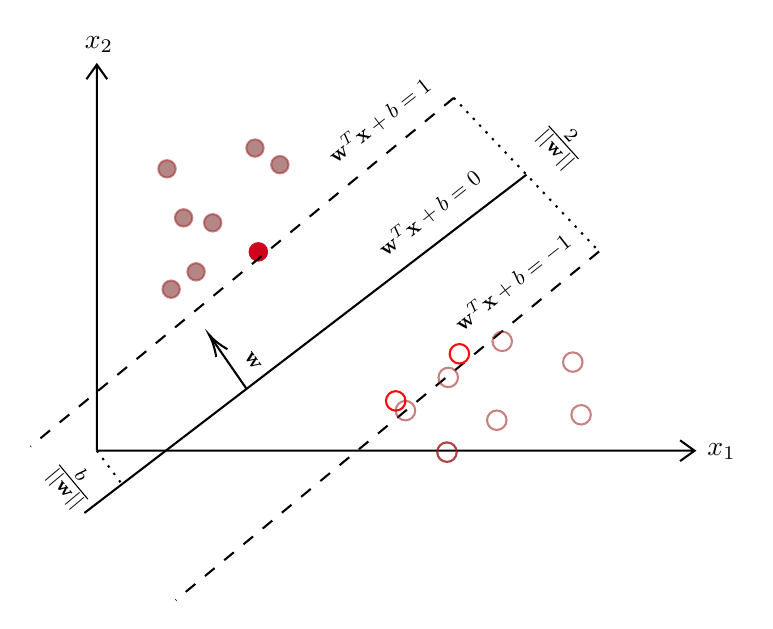
\begin{tikzpicture}[x=0.75pt,y=0.75pt,yscale=-1,xscale=1]
%uncomment if require: \path (0,635.1999969482422); %set diagram left start at 0, and has height of 635.1999969482422

%Shape: Axis 2D [id:dp8368707307276244] 
\draw  (118,248) -- (406,248)(118,62) -- (118,248) -- cycle (399,243) -- (406,248) -- (399,253) (113,69) -- (118,62) -- (123,69)  ;
%Shape: Circle [id:dp9803563806303263] 
\draw  [color={rgb, 255:red, 157; green, 44; blue, 44 }  ,draw opacity=0.55 ][fill={rgb, 255:red, 130; green, 49; blue, 49 }  ,fill opacity=0.59 ] (147.62,112.19) .. controls (147.62,109.88) and (149.49,108) .. (151.81,108) .. controls (154.12,108) and (156,109.88) .. (156,112.19) .. controls (156,114.51) and (154.12,116.38) .. (151.81,116.38) .. controls (149.49,116.38) and (147.62,114.51) .. (147.62,112.19) -- cycle ;
%Shape: Circle [id:dp700705810808914] 
\draw  [color={rgb, 255:red, 157; green, 44; blue, 44 }  ,draw opacity=0.55 ][fill={rgb, 255:red, 130; green, 49; blue, 49 }  ,fill opacity=0.59 ] (161.62,161.81) .. controls (161.62,159.49) and (163.49,157.62) .. (165.81,157.62) .. controls (168.12,157.62) and (170,159.49) .. (170,161.81) .. controls (170,164.12) and (168.12,166) .. (165.81,166) .. controls (163.49,166) and (161.62,164.12) .. (161.62,161.81) -- cycle ;
%Shape: Circle [id:dp849847638762051] 
\draw  [color={rgb, 255:red, 157; green, 44; blue, 44 }  ,draw opacity=0.55 ][fill={rgb, 255:red, 130; green, 49; blue, 49 }  ,fill opacity=0.59 ] (149.62,170.19) .. controls (149.62,167.88) and (151.49,166) .. (153.81,166) .. controls (156.12,166) and (158,167.88) .. (158,170.19) .. controls (158,172.51) and (156.12,174.38) .. (153.81,174.38) .. controls (151.49,174.38) and (149.62,172.51) .. (149.62,170.19) -- cycle ;
%Shape: Circle [id:dp8764583906667556] 
\draw  [color={rgb, 255:red, 157; green, 44; blue, 44 }  ,draw opacity=0.55 ][fill={rgb, 255:red, 130; green, 49; blue, 49 }  ,fill opacity=0.59 ] (169.62,138.19) .. controls (169.62,135.88) and (171.49,134) .. (173.81,134) .. controls (176.12,134) and (178,135.88) .. (178,138.19) .. controls (178,140.51) and (176.12,142.38) .. (173.81,142.38) .. controls (171.49,142.38) and (169.62,140.51) .. (169.62,138.19) -- cycle ;
%Shape: Circle [id:dp5507816393851739] 
\draw  [color={rgb, 255:red, 157; green, 44; blue, 44 }  ,draw opacity=0.55 ][fill={rgb, 255:red, 130; green, 49; blue, 49 }  ,fill opacity=0.59 ] (155.62,135.81) .. controls (155.62,133.49) and (157.49,131.62) .. (159.81,131.62) .. controls (162.12,131.62) and (164,133.49) .. (164,135.81) .. controls (164,138.12) and (162.12,140) .. (159.81,140) .. controls (157.49,140) and (155.62,138.12) .. (155.62,135.81) -- cycle ;
%Shape: Circle [id:dp18118849203387677] 
\draw  [color={rgb, 255:red, 157; green, 44; blue, 44 }  ,draw opacity=0.55 ][fill={rgb, 255:red, 130; green, 49; blue, 49 }  ,fill opacity=0.59 ] (202,110.19) .. controls (202,107.88) and (203.88,106) .. (206.19,106) .. controls (208.51,106) and (210.38,107.88) .. (210.38,110.19) .. controls (210.38,112.51) and (208.51,114.38) .. (206.19,114.38) .. controls (203.88,114.38) and (202,112.51) .. (202,110.19) -- cycle ;
%Shape: Circle [id:dp5205134672007141] 
\draw  [color={rgb, 255:red, 157; green, 44; blue, 44 }  ,draw opacity=0.55 ][fill={rgb, 255:red, 130; green, 49; blue, 49 }  ,fill opacity=0.59 ] (190,102.19) .. controls (190,99.88) and (191.88,98) .. (194.19,98) .. controls (196.51,98) and (198.38,99.88) .. (198.38,102.19) .. controls (198.38,104.51) and (196.51,106.38) .. (194.19,106.38) .. controls (191.88,106.38) and (190,104.51) .. (190,102.19) -- cycle ;
%Shape: Circle [id:dp9440087008079838] 
\draw  [color={rgb, 255:red, 208; green, 2; blue, 27 }  ,draw opacity=1 ][fill={rgb, 255:red, 208; green, 2; blue, 27 }  ,fill opacity=1 ] (191.62,152.19) .. controls (191.62,149.88) and (193.49,148) .. (195.81,148) .. controls (198.12,148) and (200,149.88) .. (200,152.19) .. controls (200,154.51) and (198.12,156.38) .. (195.81,156.38) .. controls (193.49,156.38) and (191.62,154.51) .. (191.62,152.19) -- cycle ;
%Straight Lines [id:da17318721660477443] 
\draw  [dash pattern={on 4.5pt off 4.5pt}]  (290,78) -- (86,246) ;


%Straight Lines [id:da3689670668981829] 
\draw  [dash pattern={on 4.5pt off 4.5pt}]  (360,152) -- (156,320) ;


%Shape: Circle [id:dp47096268150460496] 
\draw  [color={rgb, 255:red, 252; green, 11; blue, 11 }  ,draw opacity=1 ] (257.31,224) .. controls (257.31,221.41) and (259.41,219.31) .. (262,219.31) .. controls (264.59,219.31) and (266.69,221.41) .. (266.69,224) .. controls (266.69,226.59) and (264.59,228.69) .. (262,228.69) .. controls (259.41,228.69) and (257.31,226.59) .. (257.31,224) -- cycle ;
%Shape: Circle [id:dp3309189503678929] 
\draw  [color={rgb, 255:red, 252; green, 11; blue, 11 }  ,draw opacity=1 ] (288,201.31) .. controls (288,198.72) and (290.1,196.62) .. (292.69,196.62) .. controls (295.28,196.62) and (297.38,198.72) .. (297.38,201.31) .. controls (297.38,203.9) and (295.28,206) .. (292.69,206) .. controls (290.1,206) and (288,203.9) .. (288,201.31) -- cycle ;
%Shape: Circle [id:dp9268009410434288] 
\draw  [color={rgb, 255:red, 155; green, 24; blue, 24 }  ,draw opacity=0.55 ] (262,228.69) .. controls (262,226.1) and (264.1,224) .. (266.69,224) .. controls (269.28,224) and (271.38,226.1) .. (271.38,228.69) .. controls (271.38,231.28) and (269.28,233.38) .. (266.69,233.38) .. controls (264.1,233.38) and (262,231.28) .. (262,228.69) -- cycle ;
%Shape: Circle [id:dp29527861748528006] 
\draw  [color={rgb, 255:red, 155; green, 24; blue, 24 }  ,draw opacity=0.55 ] (282,248.69) .. controls (282,246.1) and (284.1,244) .. (286.69,244) .. controls (289.28,244) and (291.38,246.1) .. (291.38,248.69) .. controls (291.38,251.28) and (289.28,253.38) .. (286.69,253.38) .. controls (284.1,253.38) and (282,251.28) .. (282,248.69) -- cycle ;
%Shape: Circle [id:dp7861193375683235] 
\draw  [color={rgb, 255:red, 155; green, 24; blue, 24 }  ,draw opacity=0.55 ] (282,248.69) .. controls (282,246.1) and (284.1,244) .. (286.69,244) .. controls (289.28,244) and (291.38,246.1) .. (291.38,248.69) .. controls (291.38,251.28) and (289.28,253.38) .. (286.69,253.38) .. controls (284.1,253.38) and (282,251.28) .. (282,248.69) -- cycle ;
%Shape: Circle [id:dp9839275133514435] 
\draw  [color={rgb, 255:red, 155; green, 24; blue, 24 }  ,draw opacity=0.55 ] (342.62,205.31) .. controls (342.62,202.72) and (344.72,200.62) .. (347.31,200.62) .. controls (349.9,200.62) and (352,202.72) .. (352,205.31) .. controls (352,207.9) and (349.9,210) .. (347.31,210) .. controls (344.72,210) and (342.62,207.9) .. (342.62,205.31) -- cycle ;
%Shape: Circle [id:dp29189292391515476] 
\draw  [color={rgb, 255:red, 155; green, 24; blue, 24 }  ,draw opacity=0.55 ] (308.62,195.31) .. controls (308.62,192.72) and (310.72,190.62) .. (313.31,190.62) .. controls (315.9,190.62) and (318,192.72) .. (318,195.31) .. controls (318,197.9) and (315.9,200) .. (313.31,200) .. controls (310.72,200) and (308.62,197.9) .. (308.62,195.31) -- cycle ;
%Shape: Circle [id:dp8238430199954245] 
\draw  [color={rgb, 255:red, 155; green, 24; blue, 24 }  ,draw opacity=0.55 ] (306,233.31) .. controls (306,230.72) and (308.1,228.62) .. (310.69,228.62) .. controls (313.28,228.62) and (315.38,230.72) .. (315.38,233.31) .. controls (315.38,235.9) and (313.28,238) .. (310.69,238) .. controls (308.1,238) and (306,235.9) .. (306,233.31) -- cycle ;
%Shape: Circle [id:dp852975984243005] 
\draw  [color={rgb, 255:red, 155; green, 24; blue, 24 }  ,draw opacity=0.55 ] (346.62,230.69) .. controls (346.62,228.1) and (348.72,226) .. (351.31,226) .. controls (353.9,226) and (356,228.1) .. (356,230.69) .. controls (356,233.28) and (353.9,235.38) .. (351.31,235.38) .. controls (348.72,235.38) and (346.62,233.28) .. (346.62,230.69) -- cycle ;
%Shape: Circle [id:dp22691308040354374] 
\draw  [color={rgb, 255:red, 155; green, 24; blue, 24 }  ,draw opacity=0.55 ] (282.62,212.69) .. controls (282.62,210.1) and (284.72,208) .. (287.31,208) .. controls (289.9,208) and (292,210.1) .. (292,212.69) .. controls (292,215.28) and (289.9,217.38) .. (287.31,217.38) .. controls (284.72,217.38) and (282.62,215.28) .. (282.62,212.69) -- cycle ;
%Straight Lines [id:da1421225594894865] 
\draw  [dash pattern={on 0.84pt off 2.51pt}]  (290,78) -- (360,152) ;


%Straight Lines [id:da5777593132117835] 
\draw    (325,115) -- (112,278) ;


%Straight Lines [id:da04571283469678322] 
\draw    (190,218) -- (173.14,193.64) ;
\draw [shift={(172,192)}, rotate = 415.3] [color={rgb, 255:red, 0; green, 0; blue, 0 }  ][line width=0.75]    (10.93,-3.29) .. controls (6.95,-1.4) and (3.31,-0.3) .. (0,0) .. controls (3.31,0.3) and (6.95,1.4) .. (10.93,3.29)   ;

%Straight Lines [id:da4500585355249126] 
\draw  [dash pattern={on 0.84pt off 2.51pt}]  (118,248) -- (130,264) ;



% Text Node
\draw (342,100.22) node [rotate=-47.98]  {$\frac{2}{||\mathbf{w} ||}$};
% Text Node
\draw (193.14,204.74) node [scale=0.8,rotate=-54.78]  {$\mathbf{w}$};
% Text Node
\draw (106.02,263.64) node [rotate=-50.17]  {$\frac{b}{||\mathbf{w} ||}$};
% Text Node
\draw (253.92,88.71) node [scale=0.8,rotate=-321.71]  {$\mathbf{w}^{T}\mathbf{x} +b=1$};
% Text Node
\draw (278.08,133.29) node [scale=0.8,rotate=-321.71]  {$\mathbf{w}^{T}\mathbf{x} +b=0$};
% Text Node
\draw (318.08,166.71) node [scale=0.8,rotate=-321.71]  {$\mathbf{w}^{T}\mathbf{x} +b=-1$};
% Text Node
\draw (419,248.5) node   {$x_{1}$};
% Text Node
\draw (119,52.5) node   {$x_{2}$};


\end{tikzpicture}


\end{document}
